% \textbf{Model uczony na stałej krzywiźnie wierzechołków}

% \begin{figure}[ht]
% 	\centering
% 	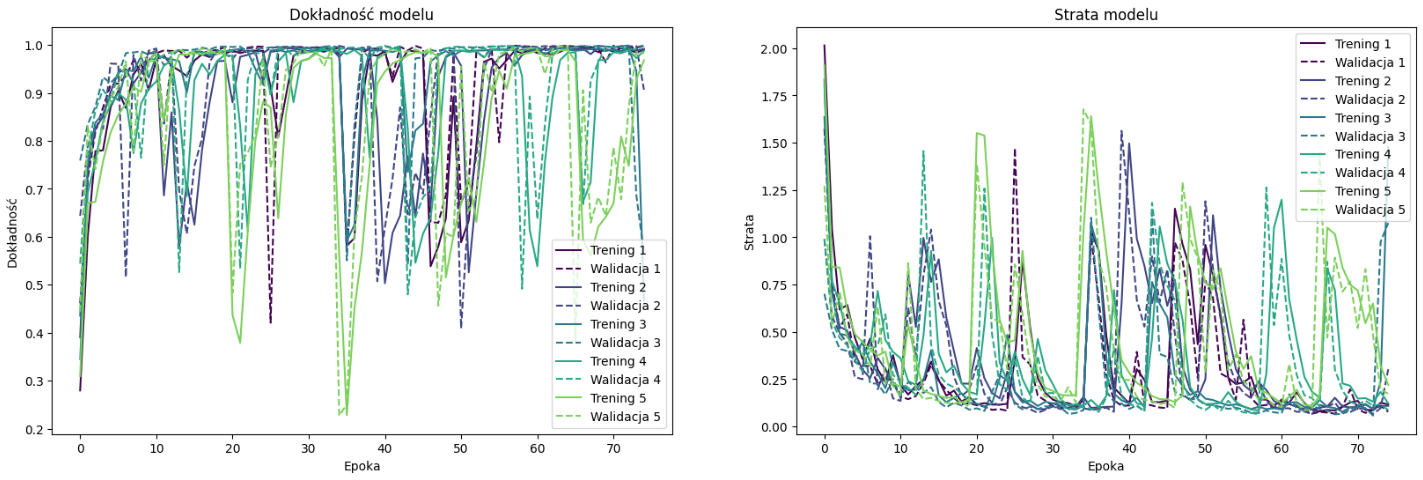
\includegraphics[height=5.5cm]{resources/tests/images/v2/crossvalid_img.png}
% 	\caption{Wyniki testów dla modelu z walidacją krzyżową i stałą krzywizną wierzechołków}
% 	\label{Fig:tests-cv-1}
% \end{figure}
% \FloatBarrier

% \begin{figure}[ht]
% 	\centering
% 	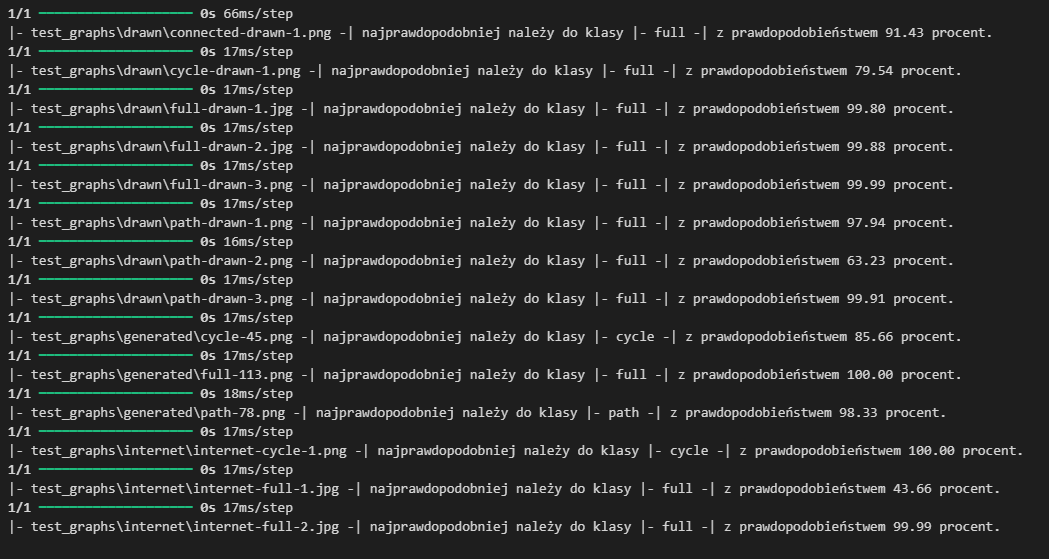
\includegraphics[height=7cm]{resources/tests/images/v2/crossvalid_txt.png}
% 	\caption{Klasyfikacja obrazów zewnętrznych dla modelu z walidacją krzyżową i stałą krzywizną wierzechołków}
% 	\label{Fig:tests-cv-2}
% \end{figure}
% \FloatBarrier

\textbf{Model uczony na losowej krzywiźnie wierzechołków}

W przypadku modelu z walidacją krzyżową, uczonego na grafach z 4 wierzchołkami,
dokładność wzrasta gwałtownie na początku treningu,
osiągając wartości powyżej 0.8 już po około 10 epokach.
Dokładność stabiliziuje się w okolicach 90\%, ale mimo to widać pewne fluktuacje, zwłaszacza na danych walidacyjnych.
Możliwe do zaobserowania są regularne spadki dokładności w niektórych epokach,
co może wynikać z niestabilnego treningu lub problemów modelu w generalizacji dla niektórych danych walidacyjncyh.

Dla straty modelu można zaobserować spadek w pierwszych 10 epokach, co mogłoby wskazywać na szybkie uczenie się modelu.
Zaraz po nim, następuje stabilizacja na niskim poziomie, z pojedynczymi skokami, głównie na zbiorze walidacyjnym.
Nieregularne wzrosty straty, podobnie jak w przypadku dokładności, mogą wskazywać na problemy z przeuczeniem.

\begin{figure}[ht]
	\centering
	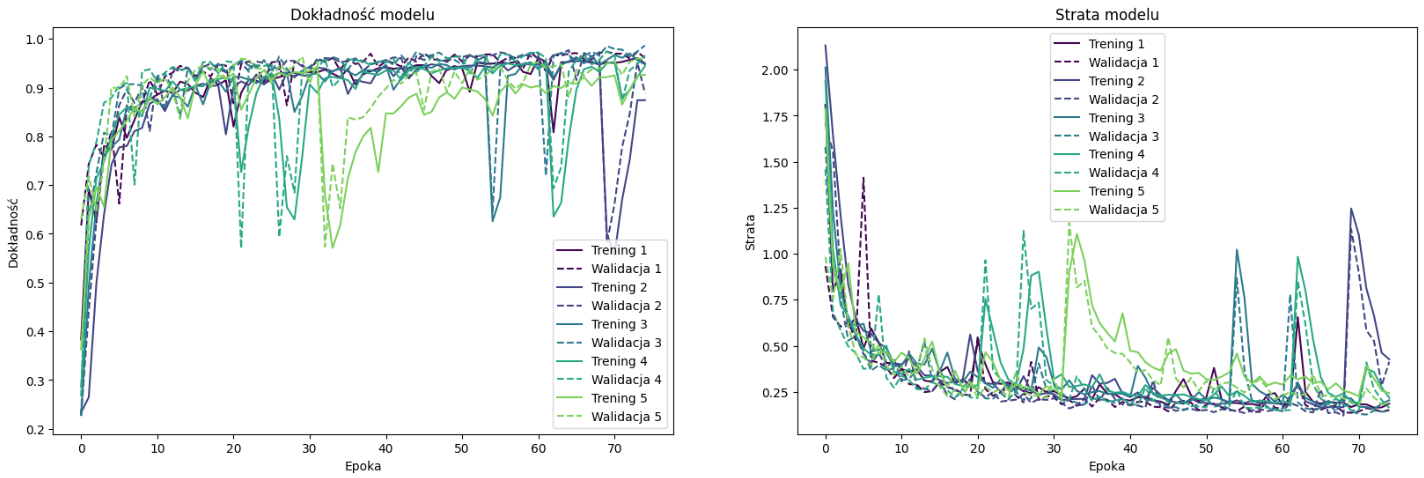
\includegraphics[height=5.5cm]{resources/tests/images/v3/crossvalid_img.png}
	\caption{Wyniki testów dla modelu z walidacją krzyżową}
	\label{Fig:tests-cv-0a}
\end{figure}
\FloatBarrier

Podsumowując, ten wariant modelu generalnie uczy się poprawnie, dzięki czemu osiąga wysoką dokładność i niską stratę.
Fluktuacje jakie występują w wynikach, szczególnie na danych walidacyjnych,
sugerują jednak potencjalne problemy z generalizacją, co może być wynikiem niestabilności modelu,
przeuczenia modelu, lub trudności w rozpoznawaniu bardziej złożonych przykładów w danych walidacyjnych.

W przypadku tego modelu, zwiększenie liczby epok, nie przyniosłoby zamierzonych skutków.
Model zbyt szybko się przeucza, a więc większa liczba iteracji nie wpłynęłaby w żaden znaczący sposób na wynik.

\begin{figure}[ht]
	\centering
	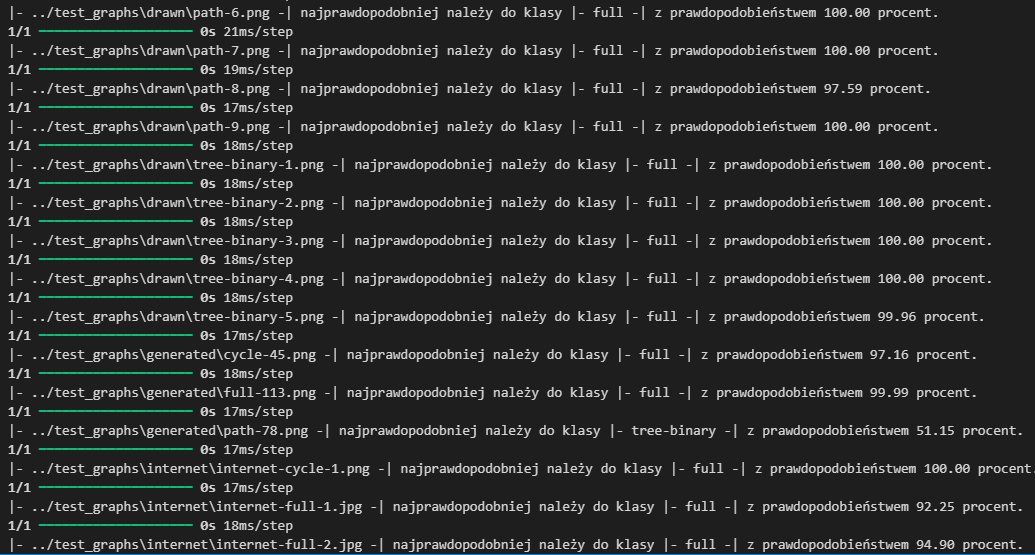
\includegraphics[height=7cm]{resources/tests/images/v3/crossvalid_txt.png}
	\caption{Klasyfikacja obrazów zewnętrznych dla modelu z walidacją krzyżową}
	\label{Fig:tests-cv-0b}
\end{figure}
\FloatBarrier

Z powodu przeuczenia model nie radził sobie z zewnętrznymi obrazkami testowymi.
Większość grafów określił jako grafy pełne, a jedną ze scieżek jako drzewo binarne,
co nie jest zgodne ze stanem rzeczywistym.

\textbf{Zmodyfikowany model}

W celu poprawy dokładności i zapobiegnięciu przeuczenia wprowadzone
zostały następujące modyfikacje do modelu z walidacją krzyżową.
Każde z nich zostało przetestowane w osobnym modelu.
Stworzony został również jeden model ze wszystkimi połączonymi modyfikacjami. 
\begin{itemize}[label=-,labelsep=0.4cm,leftmargin=0.6cm]
    \item Zmieniono liczbę filtrów w warstwach Conv2D z 32 w każdej warstwie, do kolejno 32, 64 oraz 128.
		Jednocześnie zwiększono parametr Dropout z 0,2 do 0,5.
    \item Zastosowano Batch Normalization pomiędzy warstwami modelu - konkretnie po każdej warstwie Conv2D.
    \item Wprowadzenie augmentacji danych przed budową modelu, która wprowadza więcej wariacji do zbioru treningowego,
		w celu poprawy zdolności generalizacyjnych.
		Wykorzystano również GPU w procesie prefetchingu i cachingu zbiorów danych, by przypsieszyć przetwarzanie danych.
	\item Skorzystanie z wywołania zwrotnego, które zmniejsza szybkość uczenia.
		W przypadku stagnacji dokładności w procesie przechodzenia przez kolejne epoki uczenia modelu
		może pomóc w lepszej konwergencji modelu.
\end{itemize}

\textbf{Zmodyfikowany model - Conv2D i Dropout}

\begin{lstlisting}[language=Python,caption=Listing zmodyfikowanego skryptu tworzącego model z walidacją krzyżową - wersja 1,
	label={tests-model-crossval1}]
	model = tf.keras.models.Sequential([
		tf.keras.layers.Rescaling(1./255),
		tf.keras.layers.Conv2D(32, 3, activation='relu'),
		tf.keras.layers.MaxPooling2D(),
		tf.keras.layers.Conv2D(64, 3, activation='relu'),
		tf.keras.layers.MaxPooling2D(),
		tf.keras.layers.Conv2D(128, 3, activation='relu'),
		tf.keras.layers.MaxPooling2D(),
		tf.keras.layers.Flatten(),
		tf.keras.layers.Dense(128, activation='relu', kernel_regularizer=tf.keras.regularizers.l2(0.01)),
		tf.keras.layers.Dropout(0.5),
		tf.keras.layers.Dense(len(class_names))
	  ])
\end{lstlisting}

Wszystkie przebiegi walidacji krzyżowej osiągają wysoką dokładność po kilku pierwszych epokach.
Model bardzo szybko uczy się rozpoznawać wzorce.
Walidacja również osiąga zadoalające wyniki, tj. około 90\%. Może to wskazywać na poprawną generalizację do nowych danych.
Występuje jednak niewielka niesabilność, występująca pomiędzy epokami,
co widać po gwałtownych spadkach i wzrostach dokładności walidacji.

Strata na zbiorze treningowym i walidacyjnym systematycznie maleje z kolejnymi epokami,
co może wskazywać na dobre dopasowanie do danych treningowych.
Zauważalnym problemem jest jednak spora fluktuacja obu wskaźników.
Model może napotykać trudności z pewnymi próbkami w zbiorze danych walidacyjnych. 

\begin{figure}[ht]
	\centering
	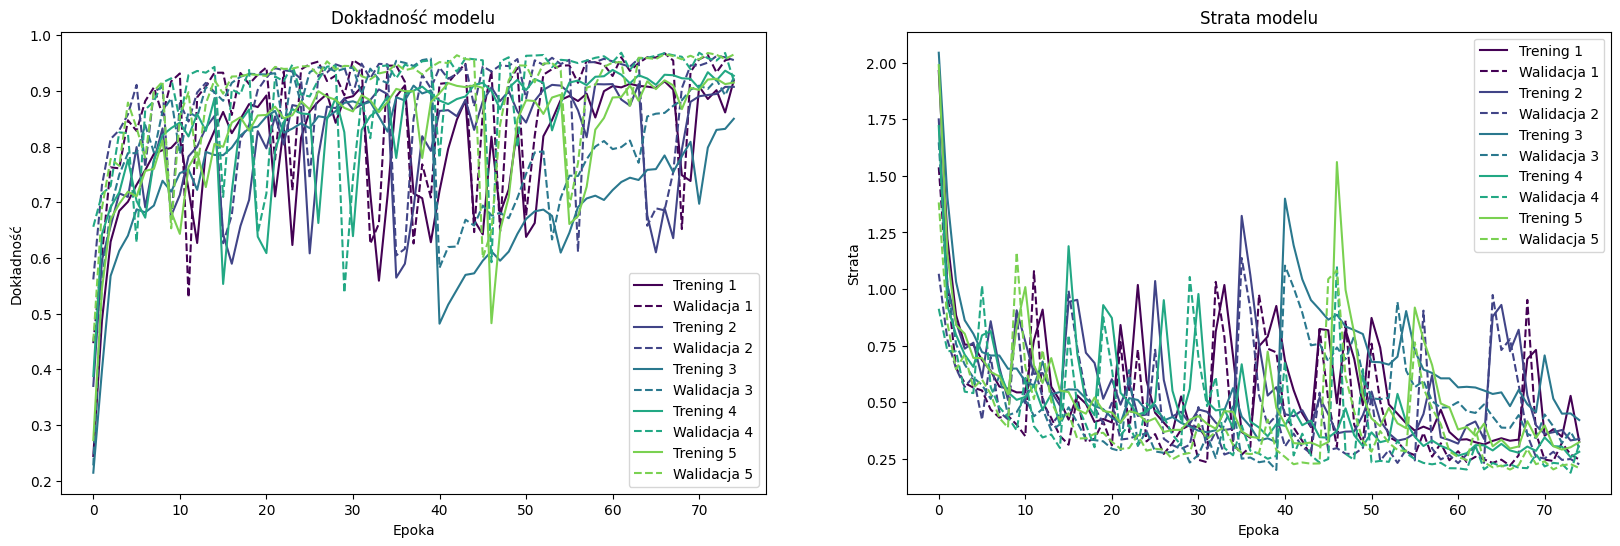
\includegraphics[height=5.5cm]{resources/tests/images/v4/crossvalid_1_img.png}
	\caption{Dokładność i walidacja dla zmodyfikowanego modelu z walidacją krzyżową - Conv2D i Dropout}
	\label{Fig:tests-cv-1a}
\end{figure}
\FloatBarrier

Modfyikacja modelu wydaje się osiągać zamierzone skutki,
ponieważ model wykazuje lepszą zdolność uczenia z danych treningowych
oraz osiąga wysoką dokładność na danych walidacyjnych.
Model może być jednak wrażliwy na trudniejsze przypadki ze zbioru danych walidacyjnych,
zważając na wahania wskaźników.

\begin{figure}[ht]
	\centering
	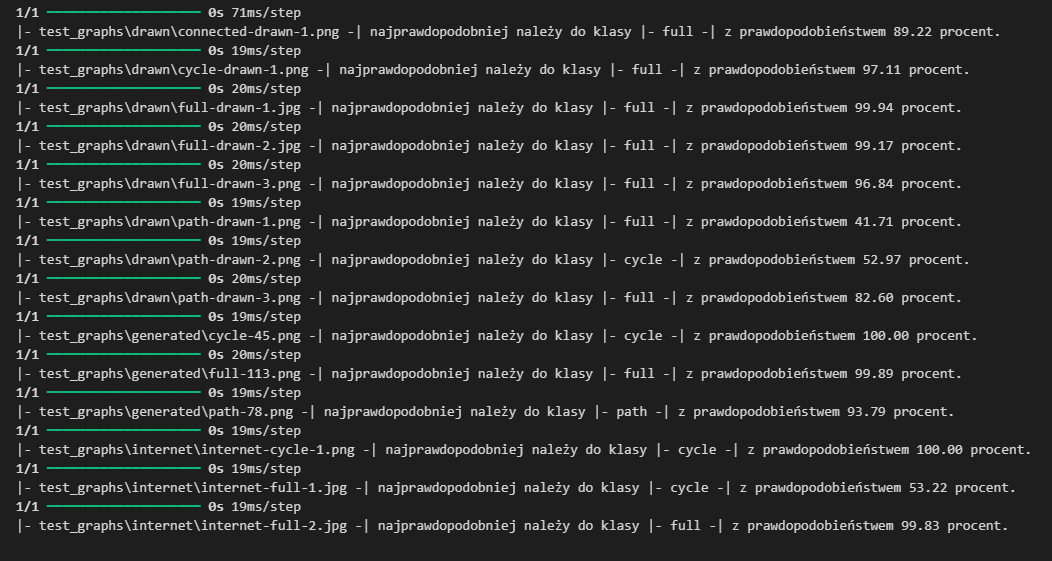
\includegraphics[height=5.5cm]{resources/tests/images/v4/crossvalid_1_txt.png}
	\caption{Klasyfikacja obrazów zewnętrznych dla zmodyfikowanego modelu z walidacją krzyżową - Conv2D i Dropout}
	\label{Fig:tests-cv-1b}
\end{figure}
\FloatBarrier

Model poprawnie sklasyfikował 9 rysunków grafów,
co jest znacznym polepszeniem w stosunku do początkowego modelu z zastosowaną walidacją krzyżową.

\textbf{Zmodyfikowany model - batch normalization}

Model został zmodyfikowany poprzez zastosowanie batch normalization pomiędzy kolejnymi warstwami Conv2D modelu.
Ma to na celu poprawienie stabilności treningu oraz przyspieszenie uczenia.
Użyte zostało również zwiększenie liczby filtrów w warstwach Conv2D oraz zwiększenie parametru Dropout
z poprzedniej modyfikacji modelu, ponieważ osięgnęła ona zamierzone cele.

\begin{lstlisting}[language=Python,caption=Listing zmodyfikowanego skryptu tworzącego model z walidacją krzyżową - wersja 2,
	label={tests-model-crossval2}]
	model = tf.keras.models.Sequential([
      tf.keras.layers.Rescaling(1./255),
      tf.keras.layers.Conv2D(32, 3, activation='relu'),
      tf.keras.layers.BatchNormalization(),
      tf.keras.layers.MaxPooling2D(),
      tf.keras.layers.Conv2D(64, 3, activation='relu'),
      tf.keras.layers.BatchNormalization(),
      tf.keras.layers.MaxPooling2D(),
      tf.keras.layers.Conv2D(128, 3, activation='relu'),
      tf.keras.layers.BatchNormalization(),
      tf.keras.layers.MaxPooling2D(),
      tf.keras.layers.Flatten(),
      tf.keras.layers.Dense(128, activation='relu', kernel_regularizer=tf.keras.regularizers.l2(0.01)),
      tf.keras.layers.Dropout(0.5),
      tf.keras.layers.Dense(len(class_names))
  ])
\end{lstlisting}

Na wykresach dokładności treningowych widać stały wzrost od około 70\% do prawie 100\%.
Jest to oczywiście pozytywna cecha modelu, lecz po analizie krzywych dokładności walidacyjnych,
należy stwierdzić, że jest to przeuczenie. Model poprawnie nauczył się danych treningowych,
lecz nie zapamiętał ogólnych wzorców, zważając na wysokie wahania oraz niestałość walidacji.

Strata treningowa, co jest spodziewane po uznaniu model za przeuczony,
osiąga bardzo niskie wartości treingowe - przez wszystkie epoki jest bliska 0.
Strata walidacyjna zaś, mimo że pozornie wygląda na stabilną, taka nie jest
- należy zwrócić uwagę na jednostki na skali. Wahania są bardzo duże oraz występuje pojedyncza wartość odstająca,
która osiąga ponad 6000 jednostek.

\begin{figure}[ht]
	\centering
	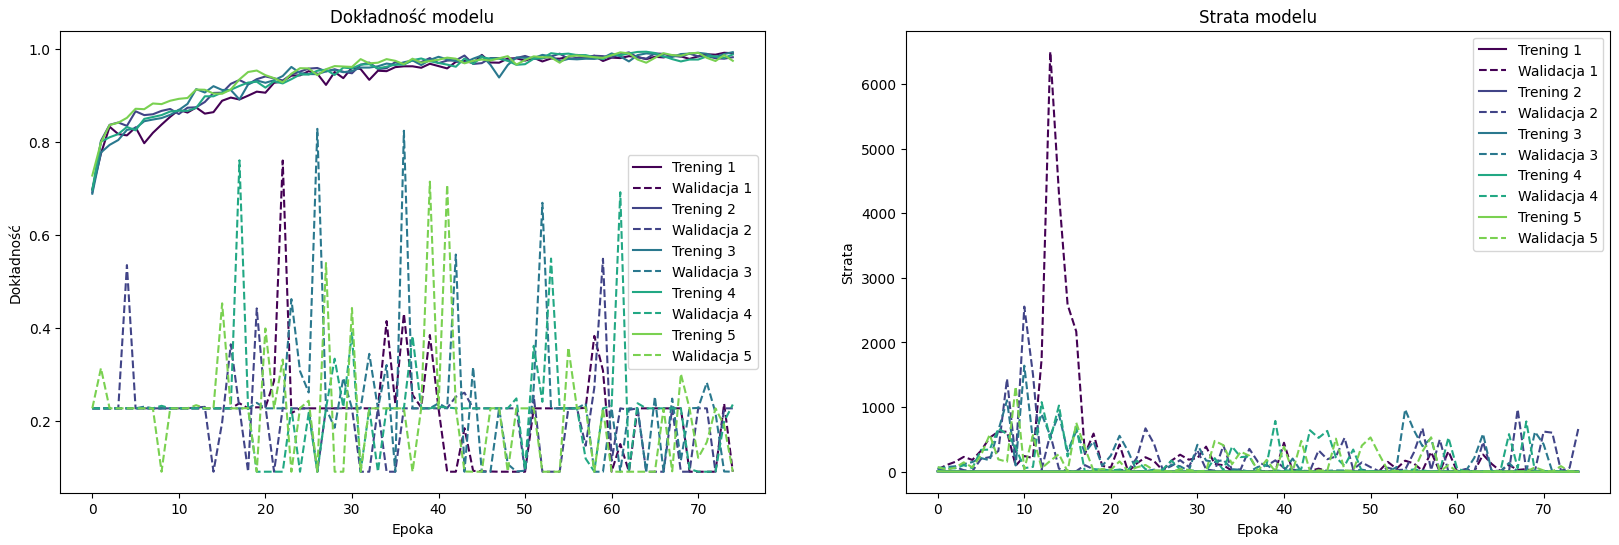
\includegraphics[height=5.5cm]{resources/tests/images/v4/crossvalid_2_img.png}
	\caption{Dokładność i walidacja dla zmodyfikowanego modelu z walidacją krzyżową - Batch Normalization}
	\label{Fig:tests-cv-2a}
\end{figure}
\FloatBarrier

Model jest nadmiernie dopasowany do danych treningowych i nie pot

\begin{figure}[ht]
	\centering
	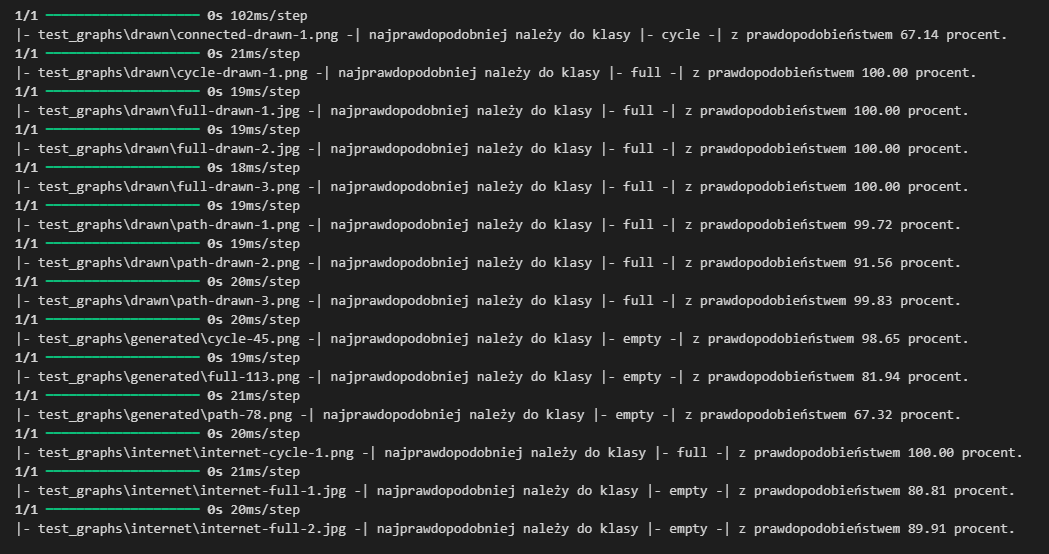
\includegraphics[height=5.5cm]{resources/tests/images/v4/crossvalid_2_txt.png}
	\caption{Klasyfikacja obrazów zewnętrznych dla zmodyfikowanego modelu z walidacją krzyżową - Batch Normalization}
	\label{Fig:tests-cv-2b}
\end{figure}
\FloatBarrier

Model sklasyfikował poprawnie tylko 3 grafy zewnętrzne. Jest to zdecydowanie poniżej oczekiwań.
Zastosowanie batch normalization nie spełniło założonej funkcji. Jest to nieudany eksperyment.

\textbf{Zmodyfikowany model - augmentacja danych}

Przed rozpoczęciem nauki modelu, zastosowana została augmentacja danych treningowych.
Najpierw, stworzony został sekwencyjny model, składający się z pewnych warstw.
Pierwsza z nich - RandomFlip, odwraca losowe obrazy w poziomie, zwiększając tym samym różnorodność danych.
Kolejna - RandomRotation, losowo obraza obrazy o kąt w zakresie od -0.1 do 0.1 radianów,
tym samym pomagając modelowi stać się odpornym na rotacje grafów.
RandomZoom z kolei przybliża lub oddala obrazy o wartości oscylujące w zakresie 10\%.
W teorii, powinno to uodpornić model na grafy różnej wielkości.
W kolejnej linii skryptu, wyżej stworzony sekwencyjny model został zastosowany do zbioru danych treningowych.
Dalej, na zbiorach uczących i walidacyjnych, użyte zostały funkcje cachujące dane - przyspiesza to proces uczenia.

\begin{lstlisting}[language=Python,caption=Listing zmodyfikowanego skryptu poprzedzającego tworzenie modelu z walidacją krzyżową
	- wersja 3,label={tests-model-crossval3}]
	data_augmentation = tf.keras.Sequential([
        tf.keras.layers.RandomFlip("horizontal"),
        tf.keras.layers.RandomRotation(0.1),
        tf.keras.layers.RandomZoom(0.1),
    ])
    train_ds = train_ds.map(lambda x, y: (data_augmentation(x), y))
    train_ds = train_ds.cache().shuffle(1000).prefetch(buffer_size=tf.data.AUTOTUNE)
    val_ds = val_ds.cache().prefetch(buffer_size=tf.data.AUTOTUNE)
\end{lstlisting}

Dokładność treningowa i walidacyjna w ciągu kilku pierwszych epok wzrasta znacząco,
od około 23\% do 50\%, po czym rośnie w stałym tempie do 90\%.
Wydają się to być dość realistyczne wartości dokładności dla nieprzeuczonego modelu.
Głównym problemem w tym przypadku wydają się być niektóre przebiegi walidacji krzyżowej.
W ich przypadku, dokładność na danych treningowych oraz walidacyjnych wynosi przez wszystkie epoki uczenia, około 23\%.
Przy każdej iteracji walidacji krzyżowej generowane są nowe zbiory walidacyjne i treningowe,
co w połączeniu z augmentacją danych, może powodować, że niektóre z tych zbiorów są wyjątkowo trudne do nauki dla modelu.
Możliwe jest również, że niektóre zbiory na których dokonano augmentacji, zważając na to, że jest ona losowa,
są nieprzystosowane do nauki modeli uczenia maszynowego.

Strata zachowuje się podobnie jak dokładność. Dla pewnych przejść walidacji krzyżowej, osiąga ona realistyczne
i spadające z biegiem epok wartości. Dla innych zaś, wartości straty są stałe przez wszystkie epoki uczenia.

\begin{figure}[ht]
	\centering
	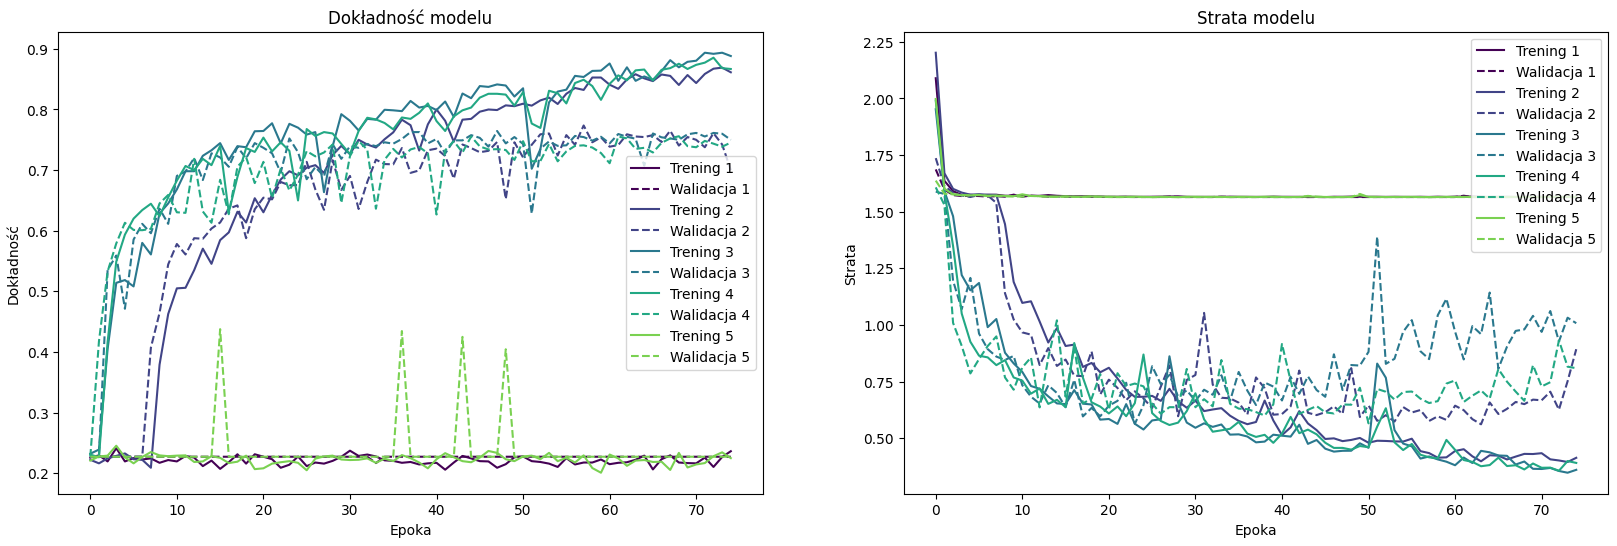
\includegraphics[height=5.5cm]{resources/tests/images/v4/crossvalid_3_img.png}
	\caption{Dokładność i walidacja dla zmodyfikowanego modelu z walidacją krzyżową - augmentacja danych}
	\label{Fig:tests-cv-3a}
\end{figure}
\FloatBarrier

Model wydaje się radzić poprawnie z niektórymi wariantami zaugmentowanych danych, a z innymi - całkowicie nie,
co wyraża się w krzywych dokładności oraz straty modelu.

\begin{figure}[ht]
	\centering
	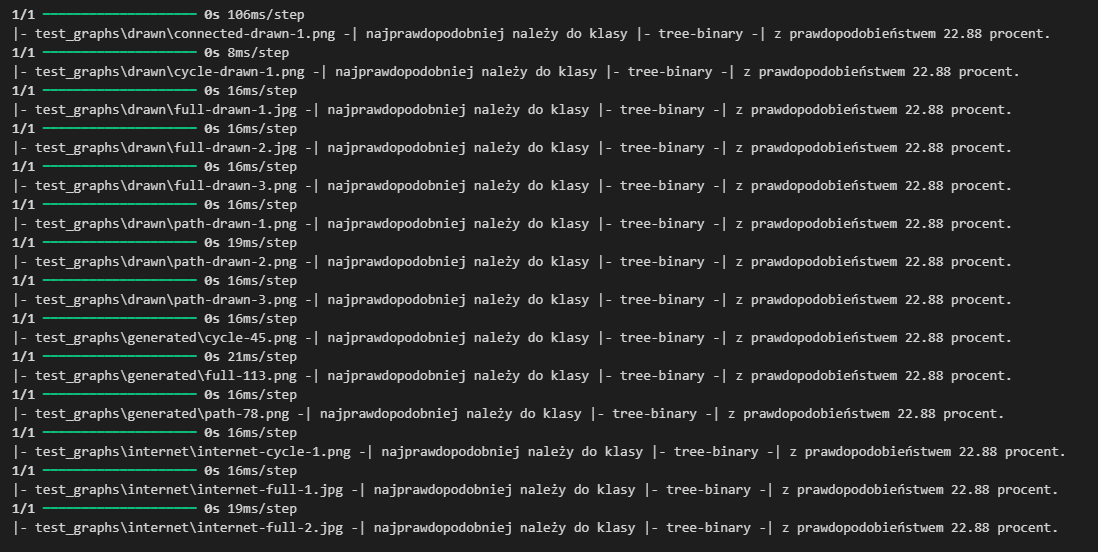
\includegraphics[height=5.5cm]{resources/tests/images/v4/crossvalid_3_txt.png}
	\caption{Klasyfikacja obrazów zewnętrznych dla zmodyfikowanego modelu z walidacją krzyżową - augmentacja danych}
	\label{Fig:tests-cv-3b}
\end{figure}
\FloatBarrier

Model w takiej postaci nie sklasyfikował poprawnie żadnego rysunku grafu.
Nie jest to zaskoczenie, mając na uwadze osiągniętą dokładność modelu na pewnych przejściach walidacji krzyżowej,
która wynosiła około 22-23\%.

\textbf{Zmodyfikowany model - spowolnienie uczenia}

Opis modyfikacji % ------ TO DO ------ %
W tym modelu zostało zastosowane wywołanie zwrotne, które spowalnia proces uczenia.
Współczynnik procesu uczenia decyduje o tym, jak duże kroki wykonuje algorytm optymalizacyjny podczas aktualizacji wag sieci neuronowej.
Gdy owy współczynnik jest zbyt duży, model może oscylować wokół minimum funkcji straty i nigdy go nie osiągnąć.
W przypadku kiedy jest zbyt mały, może prowadzić do bardzo wolnego uczenia się, czy nawet utknięcia w lokalnym minimum.
Parametr $factor$ w skrypcie decyduje o tym, o jaką wartość zredukować współczynnik uczenia,
jeśli nie nastąpi poprawa uczenia przez okres wyrażony parametrem $patience$.
$min_lr$ to minimalna wartość współczynnika uczenia, poniżej której wsółczynnik nie zostanie już zredukowany.
Zapobiega to zbyt drastycznemu zmniejszeniu learning rate, które mogłoby zahamować proces uczenia się modelu.

\begin{lstlisting}[language=Python,caption=Listing zmodyfikowanego skryptu
	znajdującego się bezpośrdenio po tworzeniu modelu z walidacją krzyżową - wersja 4,label={tests-model-crossval4}]
	reduce_lr = tf.keras.callbacks.ReduceLROnPlateau(monitor='val_loss', factor=0.2, patience=5, min_lr=0.001)
\end{lstlisting}

Krzywa dokładności treningowej oraz walidacyjnej wzrasta gwałtownie w początkowych epokach nauki.
Oznacza to, że model szybko uczy się nieskomplikowanych wzorców.
W kolejnej części procesu nauki, dokładność na obu zbiorach stabiizuje się między 90\%, a 100\%.
Z powodu widocznych sporych spadków na zbiorze walidacyjnym, można założyć pewne problemy z modelem - przeuczenie.

Podobnie jak dokładność, strata gwałtownie obniża się na początku procesu uczenia.
W kolejnych epokach dokonuje się pewna stabilizacja, lecz mimo tego widoczne są fluktuacje, szczególnie na zbiorze walidacyjnym.
Możliwe, że model jest zbyt dopasowany do specyficznych cech danych treningowych i nie generalizuje odpowiednio na nowe dane.

\begin{figure}[ht]
	\centering
	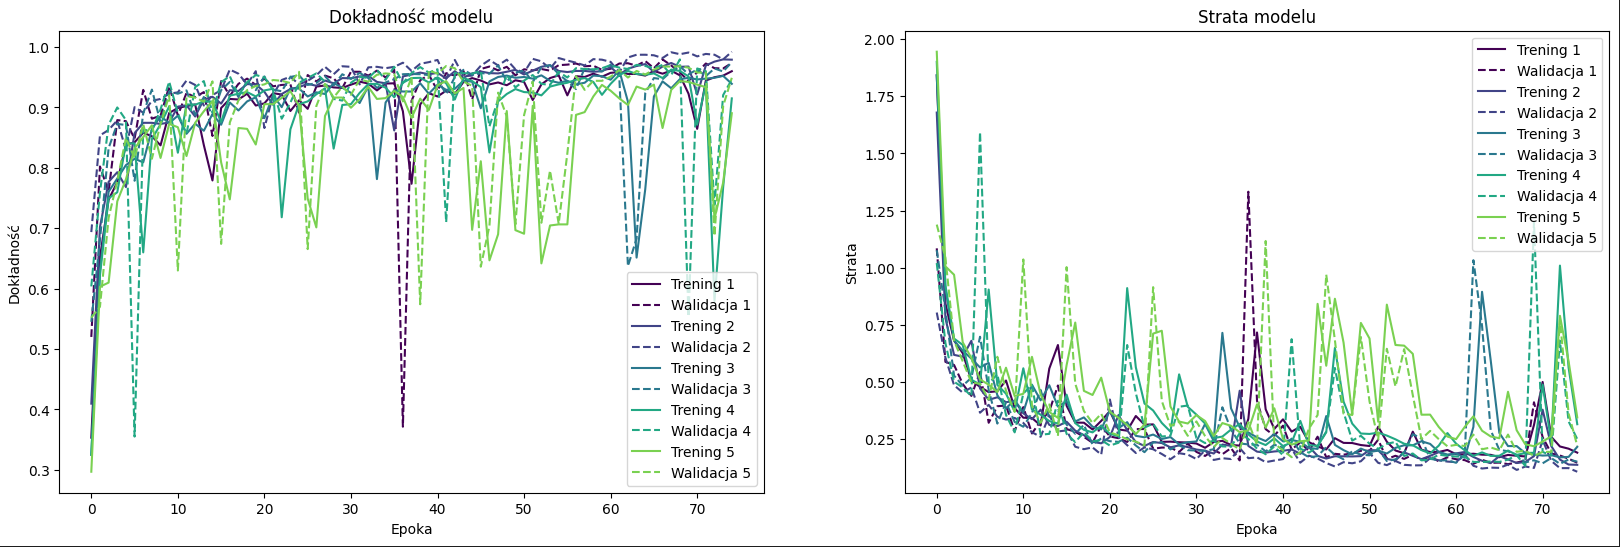
\includegraphics[height=5.5cm]{resources/tests/images/v4/crossvalid_4_img.png}
	\caption{Dokładność i walidacja dla zmodyfikowanego modelu z walidacją krzyżową - spowolnienie uczenia}
	\label{Fig:tests-cv-4a}
\end{figure}
\FloatBarrier

Model wykazuje pewne nieporządane cechy, takie jak wahania dokładności i straty na zbiorach walidacyjnych,
co wskazuje na przeuczenie modelu.

\begin{figure}[ht]
	\centering
	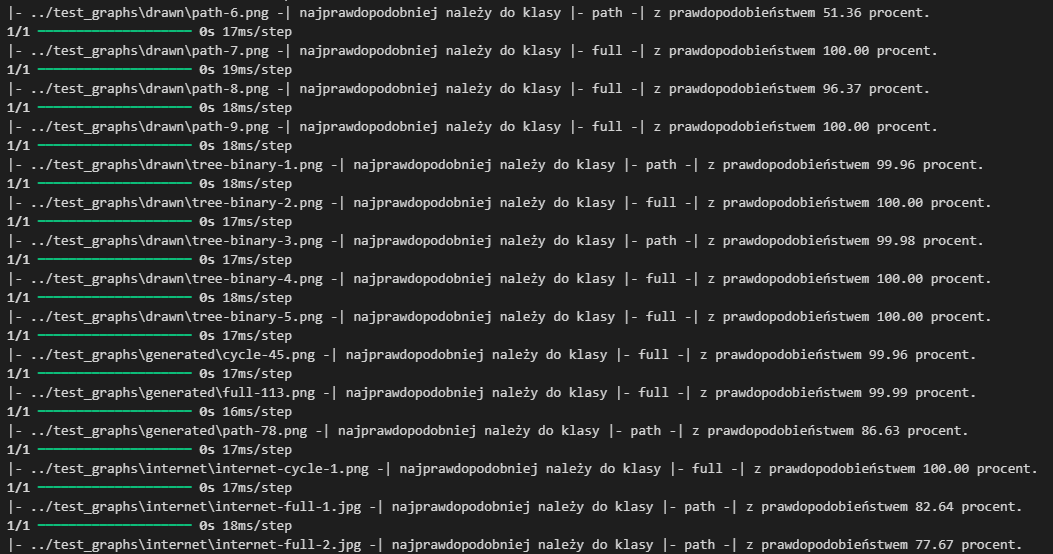
\includegraphics[height=5.5cm]{resources/tests/images/v4/crossvalid_4_txt.png}
	\caption{Klasyfikacja obrazów zewnętrznych dla zmodyfikowanego modelu z walidacją krzyżową - spowolnienie uczenia}
	\label{Fig:tests-cv-4b}
\end{figure}
\FloatBarrier

Model poprawnie sklasyfikował 6 grafów zewnętrznych.
Zważając na to, że ogólną większość grafów oznaczył jako pełne, może to również być czysty przypadek. 

\textbf{Zmodyfikowany model połączony}

Dokładność dla wszystkich przebiegów stopniowo wzrasta wraz z liczbą epok
i osiąga wysoki poziom, bo powyżej 80\%, pod koniec treningu.
W przypadku walidacji jednak, wyniki nie są zadowalające, a wrecz bardzo niestabilne.
Przez większość przebiegów uczenia utrzymuje się na niskim poziomie,
co może sugerować problemy z generalizacją danych.

Strata treningowa maleje w większości przebiegów, co jest spodziewane podczas uczenia.
Widać jednak pewne fluktuacje, świadczące o problemach z konwergencją.
Dla straty walidacyjnej można zaobserować wielką niestabilność - osiąga bardzo wysokie wartości,
nawet rzędu kilku tysięcy, jak również bardzo niskie, bliskie zeru.

\begin{figure}[ht]
	\centering
	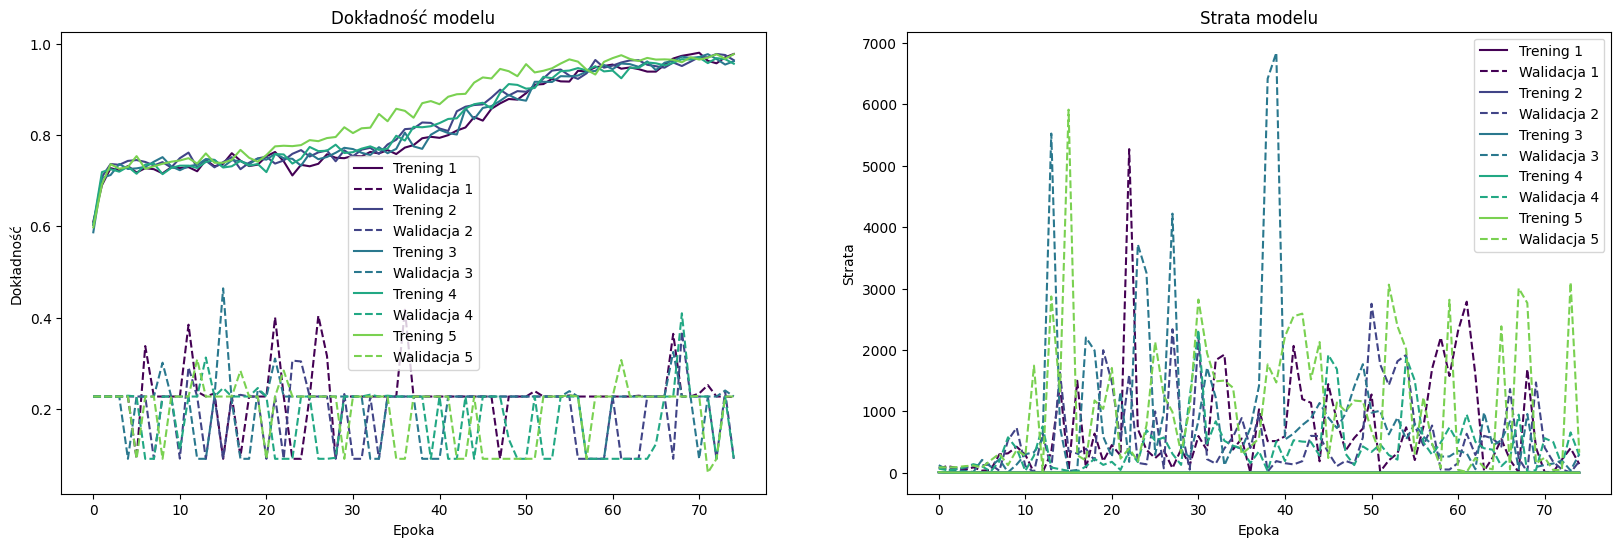
\includegraphics[height=5.5cm]{resources/tests/images/v4/crossvalid_img.png}
	\caption{Dokładność i walidacja dla zmodyfikowanego modelu z walidacją krzyżową - modyfikacja połączone}
	\label{Fig:tests-cv-5a}
\end{figure}
\FloatBarrier

Ogólne wnioski jakie można wyciągnąć z procesu uczenia tego modelu,
są takie, że model kompletnie nie radzi sobie z danymi walidacyjnymi.
Model ewidentnie przeucza się na danych treningowych,
podczas gdy jego wydajność na zbiorze walidacyjnym jest bardzo słaba.
Zastosowanie wszystkich zaproponowanych technik na raz,
nie osiągnęło zamierzonego skutku. 

\begin{figure}[ht]
	\centering
	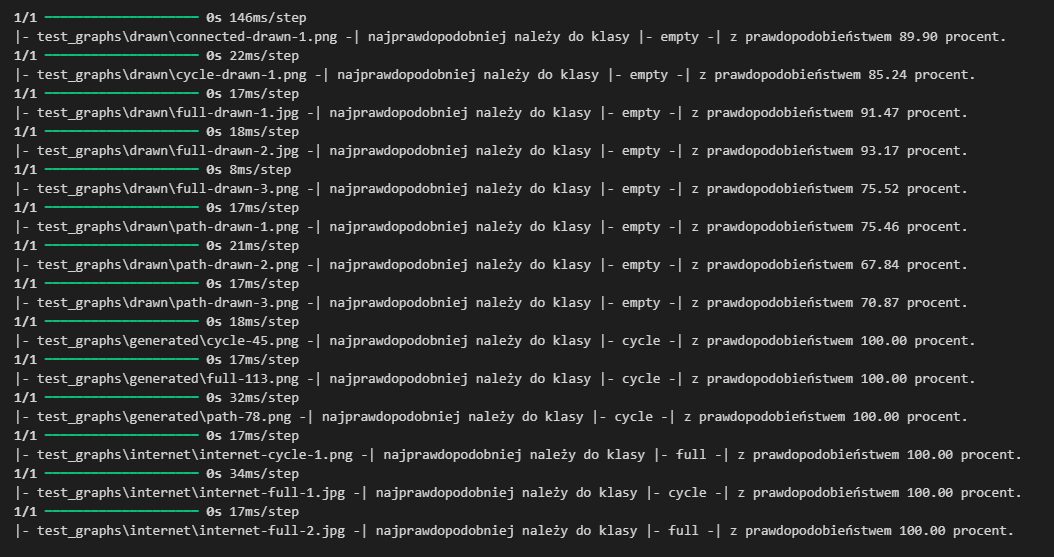
\includegraphics[height=7cm]{resources/tests/images/v4/crossvalid_txt.png}
	\caption{Klasyfikacja obrazów zewnętrznych dla zmodyfikowanego modelu z walidacją krzyżową - modyfikacja połączone}
	\label{Fig:tests-cv-5b}
\end{figure}
\FloatBarrier

Model poprawnie wskazał klasy tylko dwóch grafów testowych, co jest znacznie poniżej oczekiwanych rezultatów.